\chapter{Аналитическая часть}

\section{Анализ предметной области}

Моделирование световых эффектов гирлянды --- задача визуализации распространения света от множественных точечных источников с учетом их расположения и оптических свойств защитных элементов. Основной визуальной характеристикой гирлянды является световой узор, формируемый на освещаемых поверхностях (стенах, предметах интерьера), что требует учета физических законов геометрической оптики.

Задача моделирования гирлянд специфична из-за малых размеров источников и каустик, формируемых преломлением света в защитных колпачках. Это требует высокого разрешения расчетов и точного моделирования преломления.

Система должна обеспечивать интерактивное размещение источников, настройку параметров защитных колпачков (материал, прозрачность) и визуализацию карты освещенности после предварительного расчета.

Область применения: проектирование декоративного освещения, создание виртуальных инсталляций и демонстрация принципов геометрической оптики.

Для моделирования световых эффектов гирлянды используется геометрическая оптика, описывающая распространение света как движение лучей, подчиняющихся законам отражения и преломления \cite{1,3}. Математические модели и формулы представлены в разделе 2.2.

\subsection{Трассировка лучей как метод моделирования света}

Трассировка лучей --- метод моделирования распространения света путем отслеживания пути лучей от источников света до поверхностей или от камеры до источников света \cite{2,4}. Метод позволяет физически корректно моделировать преломление, отражение и формирование каустических эффектов.

Защитный колпачок источника света моделируется как сферический слой --- две концентрические сферы с общим центром, но разными радиусами. Источник света находится внутри малой сферы, что обеспечивает двойное преломление луча: на входе в материал (внешняя сфера) и на выходе (внутренняя сфера).

Ограничения модели:
\begin{itemize}
    \item не учитывается дисперсия света (зависимость показателя преломления от длины волны);
    \item не учитывается многократное внутреннее отражение в колпачке (только первое преломление на входе и выходе);
    \item используется упрощенная модель рассеивания (стохастическое возмущение вместо физически точных моделей микрорельефа);
    \item не учитывается поляризация света;
    \item расчет выполняется только для статической сцены (динамические эффекты не поддерживаются);
    \item модель освещения ограничена диффузным отражением (модель Ламберта), зеркальные отражения не учитываются.
\end{itemize}

\subsection{Предварительный расчет освещения}

Предварительный расчет освещения --- техника, при которой освещение рассчитывается один раз для статической сцены и сохраняется в текстуры (карты освещенности). Это позволяет достичь высокой производительности при интерактивном просмотре сцены, так как тяжелые вычисления выполняются заранее.

\section{Обзор существующих аналогов}

\subsection{DIALux evo}

Использует алгоритмы Radiosity и Ray Tracing для расчета освещенности \cite{5}. Не предоставляет средств для процедурной генерации каустических эффектов от точечных источников с учетом преломления в защитных колпачках.

\subsection{Blender (Cycles)}

Использует алгоритм Path Tracing с методом Монте-Карло \cite{6,7}. Избыточная сложность настройки каустик для точечных источников с преломляющими элементами.

\subsection{Unreal Engine 5}

Система Lumen использует гибридный подход с трассировкой лучей в реальном времени \cite{8}. Приоритет производительности над физической точностью, оптимизация для игровых сцен усложняет точное моделирование каустик от малых преломляющих элементов.

\subsection{Mitsuba 3}

Исследовательская система рендеринга, использует спектральный рендеринг \cite{9}. Управляется через скрипты, лишена графического интерфейса для интерактивной расстановки источников света.

\subsection{LuxCoreRender}

Использует Bidirectional Path Tracing \cite{10}. Низкая скорость работы (десятки минут для сложных сцен) делает невозможным интерактивную работу.

\subsection{Сравнительный анализ аналогов}

Сравнение систем проводится по критериям метода моделирования, специализации и возможности работы в режиме реального времени (после предварительного расчета).

\begin{table}[H]
\centering
\caption{Сравнительный анализ существующих решений}
\label{tab:comparison}
\begin{tabularx}{\textwidth}{|X|X|X|X|}
\hline
\textbf{Система} & \textbf{Метод расчета} & \textbf{Специализация} & \textbf{Режим работы} \\
\hline
DIALux evo & Radiosity / Ray Tracing & Инженерная светотехника & Интерактивный \\
\hline
Blender (Cycles) & Трассировка путей & 3D-анимация & Предварительный расчет \\
\hline
Unreal Engine & Трассировка лучей / предрасчет & Игры & Реальное время \\
\hline
Mitsuba 3 & Исследовательские алгоритмы & Научные исследования & Предварительный расчет \\
\hline
LuxCoreRender & Двунаправленная трассировка путей & Реалистичная графика & Предварительный расчет \\
\hline
\end{tabularx}
\end{table}

Вывод: Существующие системы ориентированы на общие задачи визуализации, что усложняет оперативную разработку дизайна декоративного освещения. 

\section{Постановка задачи}

Программа должна выполнять моделирование световых паттернов статических декоративных гирлянд с учетом физических законов геометрической оптики.

Входные данные: Конфигурация источников света (позиция, цвет, интенсивность, количество лучей), параметры защитных колпачков (радиусы, коэффициент преломления, прозрачность, рассеивание), геометрия сцены (стена, сферы), параметры камеры и расчета.

Выходные данные: Карты освещенности для стены и сфер (двумерные массивы RGB значений), изображение вида камеры.

Ограничения: Система визуализирует только эффекты освещения на поверхностях; расчет выполняется для статической конфигурации; количество источников и объектов ограничено производительностью; разрешение карт ограничено доступной памятью.

Требования к системе:
\begin{itemize}
    \item моделирование прохождения света через преломляющие среды (колпачки);
    \item формирование карт освещенности на диффузных поверхностях (стенах и объектах сцены);
    \item поддержка стохастического рассеивания для имитации матовых материалов;
    \item обеспечение интерактивного просмотра сцены за счет технологии предварительного расчета освещения;
    \item графический пользовательский интерфейс для интерактивного размещения источников света и объектов сцены;
    \item инструменты создания паттернов гирлянды (точка, линия, дуга, круг);
    \item возможность редактирования параметров источников света (позиция, цвет, интенсивность) и защитных колпачков (коэффициент преломления, прозрачность, рассеивание);
    \item интерактивное управление камерой для просмотра результатов с разных ракурсов;
    \item визуализация результатов расчета в реальном времени.
\end{itemize}

\subsection{IDEF0 диаграмма}

На рисунке \ref{fig:idef0} представлена контекстная диаграмма системы моделирования световых паттернов гирлянды (диаграмма уровня A-0).

\begin{figure}[H]
\centering
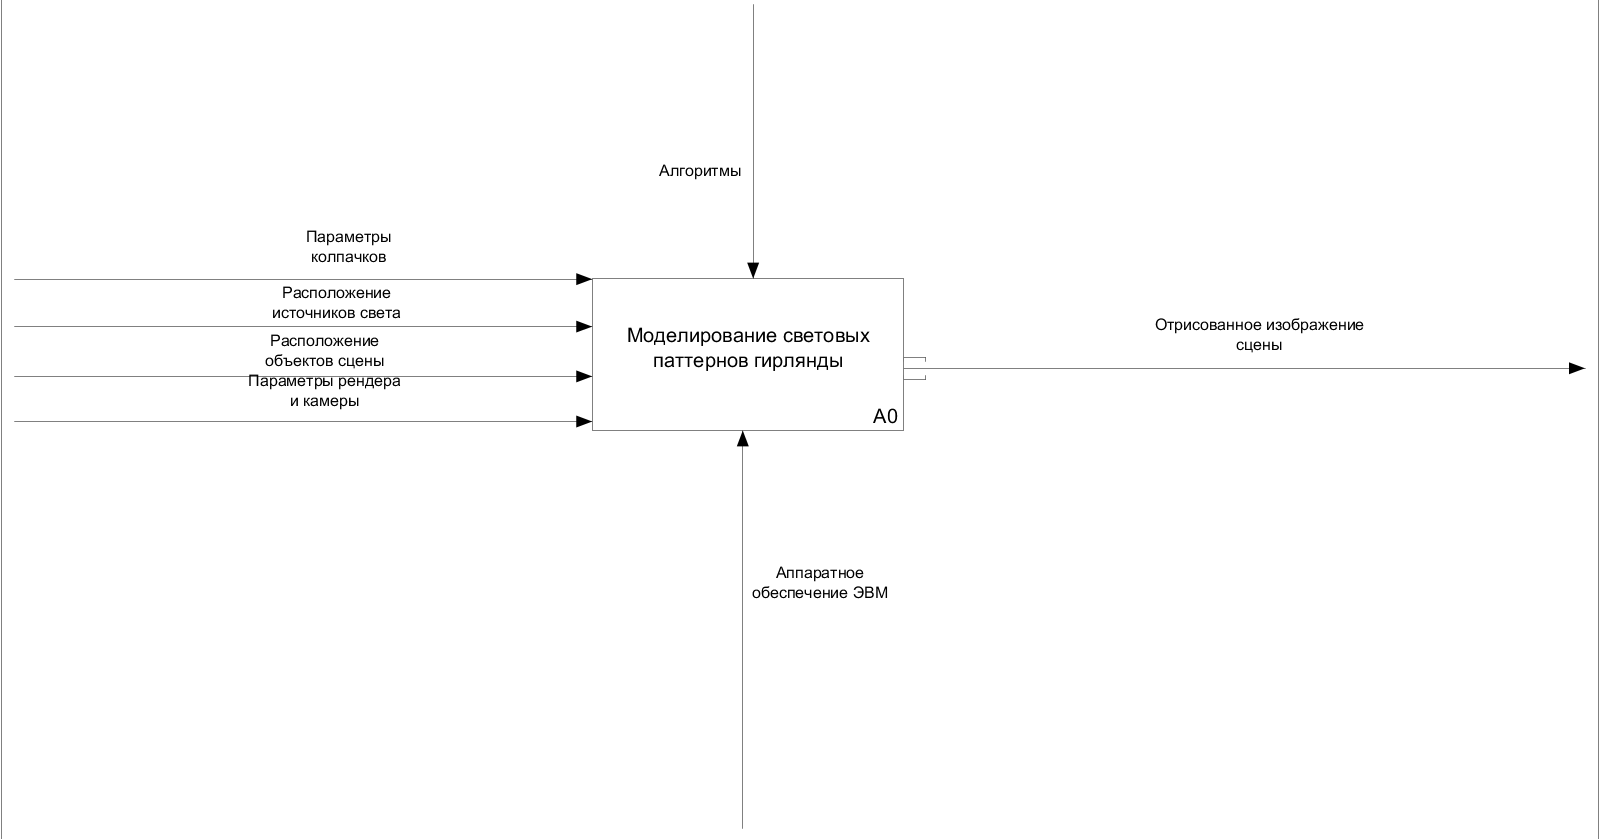
\includegraphics[width=1\textwidth]{images/01_A-0.png} 
\caption{Контекстная диаграмма системы симуляции (IDEF0 A-0)}
\label{fig:idef0}
\end{figure}

\clearpage
